\section{Hardening di base e controllo dell'accesso}

\subsection{Introduzione alla sicurezza}
E' innanzitutto bene comprendere che quando si parla di sicurezza, e' bene comprendere che quest'ultima non si realizza attraverso un particolare prodotto software o hardware acquistabile presso terzi;
\begin{center}
	``La sicurezza e' il risultato di un \textbf{processo}"
\end{center}
Bisogna infatti pensare alla sicurezza come al risultato di un processo che prende in considerazione non solo tutte gli aspetti tecnologici ma anche quelli umani. Ottenere un livello accettabile di sicurezza richiede pazienza, attenzione, conoscenza e determinazione. Vediamo qualche principio generale da tenere in considerazione quando si parla di sicurezza:
\begin{itemize}
	\item Uno dei pochi punti fermi a tal proposito e' che la sicurezza si gestisce efficacemente solo vietando qualsiasi comportamento non esplicitamente consentito. Allo stesso tempo. cio' che e' consentito deve essere svolto con i diritti piu' restrittivi e compatibili con l'esecuzione del compito.
	\item La sicurezza e' antagonista dell'usabilita': e' necessario cercare soluzioni che pongano meno ostacoli possibili fra il servizio che si vuole garantire in maniera sicura e gli utenti finali che voglioni utilizzarlo.
\end{itemize}
Il campo della sicurezza informatica e' molto ampio, ma viene spesso descritto attraverso tre parametri fondamentali, i quali compongono la famosa ``\textbf{CIA triad}":
\begin{center}
	\item Confidentiality (Riservatezza)
	\item Integrity (Integrita')
	\item Availability (Disponibilita')
\end{center}

\paragraph{Confidentiality} 
La confidenzialita' tratta la \emph{riservatezza} dei dati. L'accesso alle informazioni deve essere limitato ai soggetti autorizati. Autenticazione, controllo degli accessi e cifratura delle informazioni sono alcuni sottocomponenti che contribuiscono ad assicurare questa proprieta'.

\paragraph{Integrity}
L'integrita' rappresenta l'\emph{autenticita'} delle informazioni. Le tecnologie volte a determinare l'integrita' dei dati garantiscono che questi siano validi e non siano stati alterati in maniera non autorizzata. Affronta anche l'affidabilita' delle fonti di informazione. Quando un sito web sicuro presenta un certificato TLS firmato, garantisce all'utente non solo che le informazioni che vengono scambiate sono protette da meccanismi crittografici ma anche che un'autorita di certificazione (\emph{CA, Certification Authority}) ha verificato l'identita' della sorgente.

\paragraph{Availability}
La disponbilita' esprime l'idea che le informazioni debbano essere accessibili da soggetti autorizzati in qualsiasi momento questi ne abbiano necessita'. Altrimenti, le informazioni non avrebbero valore.
\\\\
I principi della CIA Triad ci danno una linea guida per progettare, implementare e mantenere sistemi e reti.

\subsubsection{Compromissione della sicurezza}
In questa sezione diamo un occhiata generale a quali sono i problemi legati alla sicurezza nel mondo reale. Gran parte delle modalita' con le quali e' possibile compromettere un sistema rientrano nelle seguenti categorie.

\paragraph{Social Engineering}
L'essere umano, utente (e amministratore) di un sistema e' l'anello piu' debole nella catena di sicurezza. Nessun tipo di tecnologia puo' proteggere dall'elemento umano - bisogna ssicurarsi che la propria comunita' di utenti sia fortemente sensibilizzata e abbia una grande consapevolezza delle problematiche e delle minacce legate alla sicurezza cosi' che possano diventare anch'essi parte della difesa.

\paragraph{Software Vulnerabilities}
Negli anni, sono stati scoperti una quantita' innumerevole di falle di sicurezza all'interno del software di uso comune e non. Gli hacker si sono resi abili nello sfruttarle a loro vantaggio, manipolando e compromettendo interi sistemi. In un certo senso, i sistemi di sicurezza open source hanno un vataggio in termini di sicurezza. Il codice sorgente di Linux e FreeBSD e' messo a disposizione di chiunque, e migliaia di persone possono mettersi in gioco e analizzare ogni singola riga di codice alla ricerca di un'eventuale crepa da sfruttare. Si pensa quindi che questo approccio porti ad ottenere migliori risultati in termini di sicurezza e affdabilita' del software di contro a sistemi operativi proprietari (e quindi con codici sorgenti privati), ai quali e' concesso l'accesso soltanto ad un numero limitato di persone.

\paragraph{Distributed denial-of-service attacks (DDosS)}
Un attacco di tipo DDoS punta ad interrompere o impattare negativamente le performance di un servizio, compromettendone la disponibilita' agli utenti legittimi. Questi si realizzano spesso attraverso la saturazione del traffico di rete , inondando di richieste un determinato servizio cosi' da saturare le risorse disponibili. Spesso per condurre un attacco di questo tipo gli Hacker si appoggiano a ``\emph{botnet}", ovvero intere reti di dispositivi compromessi e controllati da remoto a fini malevoli. Gran parte della responsabilita' legata alla prevenzioni di questi attacchi ricade su chi gestisce la rete. Esistono software e componenti hardware appositamente progettate per rilevare attacchi di questo tipo e contrastarli continuando a garantire la disponibilita' del servizio. Ad ogni modo queste tecnologie non sempre riescono a mitigare perfettamente questi attacchi e le minacce sono in continua evoluzione.

\paragraph{Insider abuse}
Dipendenti, terzisti e consulenti sono agenti fidati di un'organizzazione ai queli spesso vengono garantiti privilegi speciali. Spesso pero' questi privilegi vengono abusati. Interni possono rubare o rivelare informazioni, corrompere sistemi sotto pagamento, o devastare per motivi politici. Queste tipologie di attacchi sono spesso i piu' complessi da rilevare per questo motivo solo le organizzazioni piu' rigorose controllano sistematicamente i loro dipendenti.

\paragraph{Network, system, or application configuration errors}
Il software puo' essere configurato in maniera sicura o non tanto sicura. Questo viene sviluppato per essere utile e non noioso, di conseguenza spesso l'opzione ``non tanto sicura" e' quella standard. Gli hacker spesso si garantiscono l'accesso ai sistemi passando per feature considerate utili e convenienti in circostanze meno insidiose: account senza password, firewall con regole molto permissive, database non protetti, etc. Un tipico esempio di una vulnerabilita' e' la pratica standard di concedere ad un sistema linux di fare boot senza che il boot-loader richieda alcuna password. Questa mancanza apre le porte ad attacchi fisici. Comunque, e' un esempio perfetto della necessita' di trovare un equilibrio fra sicurezza e usabilita'. Richiedere una password significa impedire , in caso di reboot del sistema, il completo restart della macchina , richiedendo quindi la presenza fisica di un amministratore di sistema.

\subsubsection{Messa in sicurezza fisica}
La predisposizione fisica di un sistema ha un'\textbf{importanza rilevante}. Un server e' prima di tutto un sistema di calcolo, collocato in un ambiente e connesso a una varieta' di dispositivi. Normalmente si tende a concentrare le difese sul fronte degli attacchi via rete, a componenti software come applicazioni e sistema operativo, ma tutte queste contromisure possono essere facilmente aggirate si possiede accesso fisico al sistema. Le minacce principali in questione sono:
\begin{itemize}
	\item Furto dello storage o dell'intero calcolatore
	\item Connessione di sistemi di raccolta dati alle interfacce
	\item Avvio del sistema con un sistema operativo arbitrario
\end{itemize}
La gravita' di queste minacce dipende fortemente dallo specifico ambiente. Molti di questi problemi non si presentano piu' nello scenario comune che tende sempre piu' ad affidarsi a sistemi di virtualizzazione su Cloud gestiti esternamente, ma altri concettualmente simili sono appparsi, e la logica delle stesse contromisure si puo' adattare.
		
\subsection{Pianificare l'installazione del Sistema Operativo}
Introdotte le motivazioni per cui anche la predisposizione fisica gioca un ruolo importante nel processo di messa in sicurezza di un sistema, passiamo ora allo step successivo in un ipotetico ciclo di vita di un sistema. Dopo aver messo in piedi un hardware funzionante si procede con l'istallazione di un \textbf{sistema operativo}. 

\paragraph{Distribuzione}
Sempre per attenerci al principio del \emph{minimo privilegio} ossia non mettere in piedi niente che non sia strettamente necessario, cosi' da evitare a prescindere che venga utilizzato, il sistema che si vuole impiegare in questi casi e' un sistema ``ridotto all'osso", ovvero con la minima quantita' di utility e software essenziali al lavoro che la nostra macchina dovra' poi svolgere. Questa filosofia non si rispecchia molto nelle distribuzione che troviamo normalmente in circolazione che spesso , insieme all'installazione del sistema operativo, si comprendono un set di programmi e di utility molto vasto per venire in contro a quelle che potrebbero essere le varie esigenze di un utente finale.  Questo pero' non e' sempre fattibile, in particolar modo per quanto riguarda i sistemi operativi in ambito aziendale, se si necessita di un supporto commerciale alla distribuzione linux che si vuole impiegare si puo' scegliere solo fra un gruppo ristretto di alternative (\emph{Red Hat, Canonical, SUSE}), dipendendo da quelle che sono invece le distribuzioni messe a disposizione cosi' come sono state certificate dal fornitore , andando poi a vedere cosa si puo' togliere per arrivare a rispecchiare le nostre esigenze.

\subsubsection{Organizzare dati e software}
Un altro aspetto sicuramente di notevole importanza , in particolare orientato ad un discorso di scalabilita' e sicurezza, e' l'organizzazione dello spazio di memorizzazione. Il concetto di partizionamento di un dispositivo di memorizzazione la fa da padrone. 
\\\\
Storicamente si tendeva a partizionare varie aree dello stesso sistema (filesystem) in base alla loro funzione in piu' filesystem e relativi dispositivi di memorizzazione in quanto le probabilita' che un disco potesse corrompersi erano significative. In questa maniera si cercava di limitare il danno ad una singola porzione del sistema, garantendo che le altre , in particolare quella contenente i file di boot e configurazione di sistema , rimanessero accessibili e quindi fosse possibile comunque far partire le opportune procedure di ripristino e salvare quel che non e' stato soggetto a guasti (a patto che non fossero proprio queste ultime a corrompersi). Al giorno d'oggi questo criterio continua ad avere una sua validita' in particolare per limitare danni dovuti alla saturazione delle risorse. Se infatti si vanno a collocare in contenitore rigidamente separati dati di tipologie diverse (\emph{Dati critici per il sistema, dati utenti, dati temporanei, etc}) il fatto che una di queste partizioni si suscettibile ad eventuali DoS e saturazioni non va ad influenzare la disponibilita' di altre funzionalita' del sistema. Questo d'altro canto risultava essere anche un lavoro molto complesso e delicato per il sistemista che doveva configurare di dischi, ovvero scegliere con cura come disporre le diverse partizioni su un hardisk perche' poi cambiarle era praticamente impossibile. 
\\\\
Fortunatamente questo tipo di limitazioni sono stati oggi superate anche grazie a sistemi come \textbf{LVM} (\emph{Logical Volume Manager}) che permettono di gestire lo spazio in maniera totalmente flessibile. E' sempre importante notare pero', come ogni volta che vado ad introdurre layer nuovi che apportano ulteriori elementi di complessita cio' non sia mai gratis; si ha infatti un impatto sulle prestazioni , che nel caso di LVM e' sostanzialmente trascurabile, ma anche un impatto sulla robustezza, dovuta al fatto che ogni qual volta si va a complicare un meccanismo, la probabilita' che uno degli ingranaggi si inceppi aumenta proporzionalmente al numero di ingranaggi introdotti. All'opposto, quindi se voglio evitare di apportare complessita', ci sono anche soluzioni molto rigide ad esempio posso configurare i miei sistemi in maniera tale che i dati veramente critici siano su dispositivi di sola lettura e che quindi siano resi sostanzialmente del tutto inalterabili.

\subsubsection{Partizionamento}
Un disco puo' essere visto banalmente con una stringa lunga di byte, essendo questi molto grandi, indirizzare il singolo byte sarebbe totalmente inutile, si tende racchiundere questi byte all'interno di \textbf{blocchi} numerati di dimensione fissa, generalmente blocchi da 4096 Byte (4KB). 
Possiamo quindi di fatto definire un disco come una sequenza di blocchi numerati. Dentro una di queste sequenze di blocchi numerati , ovvero dentro quello che chiamiamo un \textbf{block device} (\emph{dispositivo a blocchi}) e' possibile creare un \textbf{filesystem} attraverso un'operazione di \emph{formattazione}. 

\paragraph{Filesystem}
Possiamo pensare al filesystem come ad una struttura e un insieme di regole logiche per manipolare e organizzare in un albero gerarchico di diverse cartelle gruppi di dati (files) con la possibilita' di fare riferimento a questi attraverso dei nomi simbolici. Questa possibilita' viene concretizzata attraverso una mappatura tra nome logico e posizione fisica del dato associato. Tutti i filesystem hanno una caratteristica, cioe' danno per scontato che il contenitore (block device) che hanno a disposizione da organizzare sia privo di buchi, ovvero una sequenza di blocchi contingua. Sulla base di questa ipotesi e' possibile suddividere il block device in una serie di sotto-contenitori che dal punto di vista astratto risultano essere dei veri e propri dischi indipendenti.
\\\\
Il \textbf{processo di partizionamento} consiste quindi nel partire da un dispositivo a blocchi che ci mette a disposizione un elenco di blocchi disponibili, fisici, e nel suddividerlo in sottoinsiemi \textbf{contigui} di blocchi all'interno di ognuno dei quali vige una numerazione locale. Questa viene realizzata semplicemente attraverso una tabella che associa ad ogni partizione un identificativo (numero ordinale), il range di blocchi allocato (blocco di partenza e fine) e la tipologia della partizione, ovvero un'etichetta che ha prettamente un uso orientativo. 
Ogni partizione ``vive" in un mondo logico totalmente separato dalle altre. Questo significa che quando vado a formattare una di queste partizioni, posso creare filesystem di tipologie totalmente diverse, all'interno delle quali l'organizzazione dei dati non influisce su quella delle altre. Ogni partizione ha una sua dimensione massima che non puo' essere ecceduta dal filesystem. Nel caso abbia creato due partizioni distinte una per i dati utente e una per i file di sistema, la saturazione della prima non impedisce il corretto funzionamento del sistema, ma impedira' agli utenti di allocare nuova memoria per nuovi file.
\begin{wrapfigure}{R}{6cm}
	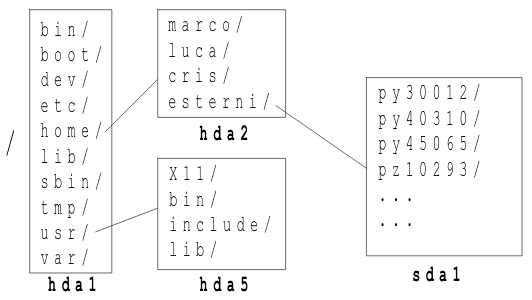
\includegraphics[scale=0.5]{"img/partitioning.png"}
	\caption{Lo schema in figura rappresenta la partizione:
		\\\\
		\begin{tabular}{ll}
			\textbf{Partizione} & \textbf{Mount point} \\
			\texttt{/dev/hda1} & \texttt{/}\\
			\texttt{/dev/hda2} & \texttt{/home/}\\
			\texttt{/dev/hda5} & \texttt{/usr/}\\
			\texttt{/dev/sda1} & \texttt{/home/esterni/}
		\end{tabular}}
\end{wrapfigure}
\paragraph{Linux} 
Linux identifica le partizioni attraverso dei file speciali con del tipo \texttt{/dev/sd*}. I file in \textbf{\texttt{/dev/}} sono \emph{block special} o \emph{character special}, cioe' non sono file che contengono dati, ma punti di accesso ai divice driver del sistema operativo, in particolare i primi adatti per l'accesso a blocchi di dati su dispositivi buffered (come appunto i dischi), i secondi per l'accesso a carattere a dispositivi come le porte ed i serial-bus. Oltre ai dispositivi fisici, un block device puo' rappresentare il punto d'accesso ance a dispositivi logici che si comportano allo stesso modo, ad esempio volumi RAID, LVM o di rete.
Ogni volta che creo un filesystem all'interno di una partizione, nella gerarchia complessiva del filesystem UNIX dovro' scegliere un \emph{mountpoint}, ovvero un punto di montaggio, che rappresentera' poi la mia via d'accesso verso quest'ultimo. 
\\\\
\paragraph{Filesystem Hierarchy Standard, FHS}
E' uno standard che definisce la struttura delle directory e relativo contenuto nei filesystem UNIX allo scopo di rendere piu' facili a programmi automatici ed utenti l'individuazione delle risorse, rendere piu' efficiente la condivisione di parti del filesystem e rendere piu' sicura la memorizzazione dei dati.
Le distinzioni di base che gidano alla corretta collozione dei dati in FHS sono 2:
\\
\begin{center}
\begin{tabular}{|l|l|l|}
	\hline
	& Condivisibili & Non condivisibili \\\hline
	Statici & es. \texttt{/usr} \texttt{/opt} & es. \texttt{/etc} \texttt{/boot} \\\hline
	Variabili & es. \texttt{/var/mail} \texttt{/var/spool/news} & es. \texttt{/var/run} \texttt{/var/lock} \\\hline
\end{tabular}
\end{center}
\\
\paragraph{Approfondimenti} Sezione \ref{filesystem}.


\subsubsection{Booting}
Una volta pianificata con attenzione la collocazione dell'hardware e la disposizione delle risorse, completiamo l'istallazione del sistema operativo e procediamo verso un primo avvio completo del sistema. Questa procedura attraversa \textbf{4 macro fasi} fondamentali:

\begin{figure}[H]
	\centering
	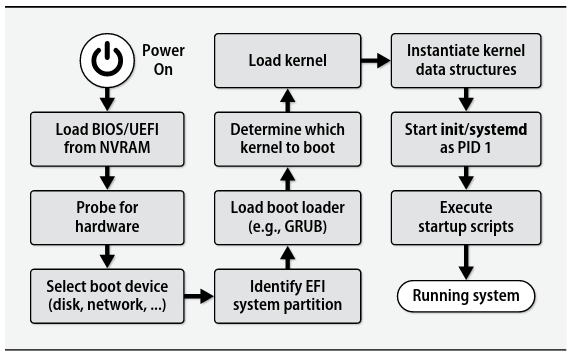
\includegraphics[scale=1]{img/linuxunixbootprocess.png}
	\caption{Linux and UNIX boot process}
\end{figure}

\paragraph{First-stage (Finding, loading, and running bootstrapping code)}
Sulla mainboard deel nostro sistema e' installata una memoria non volatile read-only (EPROM, flash*) all'interno della quale e' presente del codice, anche detto (\textbf{firmware}), tradizionalmente noto come \textbf{BIOS} (\emph{Basic Input Output System}), oggi ormai superato da un nuovo standard: \textbf{UEFI} (\emph{Unified Exstensible Firmware Interface}). 
\\
Il firmware, prodotto e preinstallato direttamente dal costruttore della scheda, e' in grado di agire a livello macchina consentendo di fare un inventario e configurare i dispositivi hardware installati sul sistema (\emph{Controller SATA, interfacce di rete, controller USB, sensori di potenza e temperatura}), potendo inoltre decidere se esporli, disabilitarli o nasconderli al sistema operativo. Consente inoltre di individuare da quali di questi possa eventualmente essere caricato ulteriore software, fare degli health-check per verificarne il corretto funzionamento, scegliere (attraverso un ordine configurabile) quale e' piu' opportuno e mandare in esecuzione lo step sucessivo.
Il BIOS si articola in due parti principali memorizzate entrambe in memorie non volatili, una che il vero e proprio firmware e l'altra si compone di tutta una serie di parametri di configurazione modificabili dall'amministratore di sistema attraverso un'interfaccia alla quale si accede premendo una combinazioni di tasti che varia in base al produttore e al modello dell' hardware (\texttt{F2, F8, F12}).

\paragraph{Second-stage (Finding,loading, and running the OS kernel)}
Il secondo step, nella procedura di avviamento del sistema, passa attraverso una seconda componente software, distinta da entrambi BIOS/UEFI e kernel del sistema operativo, che prende il nome di \textbf{Boot Loader}. Il compito principale di questo e' identificare e caricare il kernel appropriato del sistema operativo. Molti questi presentano anche un'interfaccia utente a boot-time che permette di selezionare, fra quelli presenti sul sistema, quale dei kernel o sistemi operativi mettere in esecuzione. Il fatto che questo sia un componente separato dal BIOS/UEFI e' dato dalla quantita' e varieta' di parametri necessarie a gestire e configurare l'avvio di un sistema operativo; sarebbe infatti impensabile inserire la ``consapevolezza" di tutti questi parametri e l'intelligenza per sceglierli correttamente all'interno BIOS che e' software che viene inserito in una mainboard lato produzione e mai piu' aggiornato per svariati anni essendo questo un elemento critico per la stabilita' del sistema, che contiene quindi solo gli elementi essenziali al funzionamento/interazione con la componente hardware del sistema.

\paragraph{Third-stage (Running startup scripts and system deamons)}
Una volta caricato il kernel ed eseguite le routine di inizializzazione, quest'ultimo avvia un serie di processi complementari ``spontanei" (in quanto avviati autonomamente dal kernel). Gran parte di questi sono parte dell'implementazione stessa del kernel e non per forza trovano corrispondenza in file all'interno del filesystem;e' possibile riconoscerli attraverso il comando \texttt{ps aux} da loro \texttt{PID} basso e le parentesi \texttt{[process-name]} attorno al nome del processo.
\\
Il kernel e' di per se un processo vero e proprio, con la caratteristica che essendo il primo processo ad essere effettivamente eseguito, quando il processore e' ancora in \emph{kernel-mode}, prende completo possesso del sistema e puo' procedere al caricamento dei vari device driver etc\dots creando quell'ambiente all'interno del quale e' poi possibile lanciare processi con privilegi fisici limitati (\emph{user-mode}). Il demone di amminsitrazione di sistema (\emph{system management deamon}), prende generalmente il nome di \textbf{init} e ha \textbf{process ID 1}. Il sistema concede ad \emph{init} un paio di privilegi speciali, ma per la restante parte e' un programma a livello utente esattamente come qualsiasi altro demone.

\newpage
\paragraph{Fourth-stage (Maintaining process hygiene and managing system state transitions)}
A questo step la macchina e il sistema operativo sono configurati. Il processi init si occupera' di gestire i \emph{runlevel} e i \emph{target} per coordinare l'inizializzazione del sistema, ovvero avviare i servizi nell'ordine corretto. Fara' quindi partire tutte le varie utility messe a disposizione dello user per iniziare ad utilizzare il sistema, ad esempio: il processo di \texttt{login} , eventuali ambienti grafici, etc\dots



\subsubsection{Sicurezza}
Ognuno di questi passi, dell'ottica di voler rendere sicuro il sistema, puo' essere protetto:
posso infatti stabile quali di questi step possano essere eseguiti autonomamente e quali invece richiedano l'inserimento di credenziali di autorizzazione per poter deviare dall'ordine predefinito delle cose. Il BIOS , ad esempio, puo' essere protetto da password, prestando attenzione al fatto che esistono dei meccanismi di reset in grado di ripristinarle a valori di default (purche' si abbia accesso fisico alla macchina). Lo stesso vale per il Boot Loader, e' possibile proteggere quest'ultimo con delle password. E' bene notare che questi meccanismi creano dei possibili problemi di disponibilita' non indifferenti, in quanto ad ogni riavvio (volontario o non) del sistema e' necessaria la presenza di un amministratore perche' quest'ultimo possa completare la procedura inserendo le varie credenziali. Per facilitare questo meccanismo, e' possibile impostare BIOS e Boot Loader in modo che richiedano delle credenziali solo nell'eventualita' in cui il processo di boot venga modificato rispetto a quello standard stabilito.
Sempre in termini di sicurezza, occurre notare che svariati sistemi operativi offrono una modalita' di esecuzione particolare (\emph{maintenance mode}) pensata per fare recovery in situazioni critiche, che al contempo e' possibile sfruttare per ottenere privilegi elevati all'interno di un sistema.
\\
\paragraph{Affidabilita' del software}
A questo punto dovremmo aver garantito nel percorso che va dall'accensione attraverso il pulsante \emph{power-on} al caricamento del sistema operativo, venga rispettata una sequenza prestabilita , ma non abbiamo preso in considerazione l'aspetto che concerne l'integrita', l'autenticita' e quindi l'affidabilita' del software che stiamo avviando. Partendo dall'alto, per quanto riguarda la sicurezza dei programmi che eseguiamo quotidianamente ci si affida generalmente ad un \textbf{Antivirus} o anti-malware di vario genere che hanno il compito di verificare l'integrita' delle applicazioni. A questo punto pero, bisogna considerato che l'antimalware e' un software che risiede un un disco fisico e che quindi per natura e' strutturalmente modificabile, 
\begin{center}
	\emph{chi verifica allora che questo stia effettivamente eseguendo il proprio compito o non sia stato modificato per tacere di fronte a comportamenti anomali?} \\
	Lo verifica chi lo installa e lo esegue, ovvero il \textbf{sistema operativo}. 
\end{center}
Se avessi a disposizione un sistema operativo \emph{trusted}, allora potrei quasi considerare inutile l'antimalware, ma non e' questo il caso. L'unico modo che abbiamo per avere una visione completa del sistema e' chiedere al sistema operativo, ovvero la nostra interfaccia a tutte le funzionalita' e l'hardware messo a disposizione dalla macchina. Se quest'ultimo fosse anch'esso danneggiato o compromesso, la visione di cio' che realmente sta accadendo sarebbe irrimediabilmente falsata. Abbiamo quindi la necessita' che il sistema operativo sia integro, autentico e affidabile. 
\begin{center}
	\emph{Chi verifica quindi che il sistema operativo che stiamo mettendo in esecuzione sia affidabile?}
\end{center}
Potrebbe farlo il Boot Loader, ma a questo punto ritorneremmo punto a capo, non potendo garantire che anche quest'ultimo non sia effettivamente stato corrotto. Lo stesso discorso, con tutte le complicazione tecniche del caso, vale per il BIOS.

\paragraph{Chain of trust}
L'unica cosa a cui effettivamente possiamo agganciarci per essere certi che non siano state fatte delle modifiche non autorizzate a tutta questa catena che parte dal bios fino alle applicazioni e' un dato che sia fisicamente \textbf{inalterabile}; cio' non puo' essere fatto a partire da un dato che e' scritto in un dispositivo, ad esempio un disco, che per sua natura e' fisicamente modifibile. Serve una quindi una \textbf{root of trust} (\emph{radice di fiducia}) aggianciata all'hardware: qualcosa di fisico che non possa essere \textbf{mai modificato} e al contempo possa essere \textbf{verificato}, e mi permetta di avviare una \textbf{catena di fiducia}. Se io so che il primo step dei 4, e' verificato partendo da un termine di paragone inalterabile, assolutamente affidabile, allora e' possibile propagare gli eventuali controlli di autenticita' ed integrita' su tutta la catena.

\subsubsection{Paradigmi di trusted boot}
Questa catena di fiducia nei sistemi moderni puo' essere implementata secondo due paradigmi diversi:

\begin{wrapfigure}{R}{6cm}
	\centering
	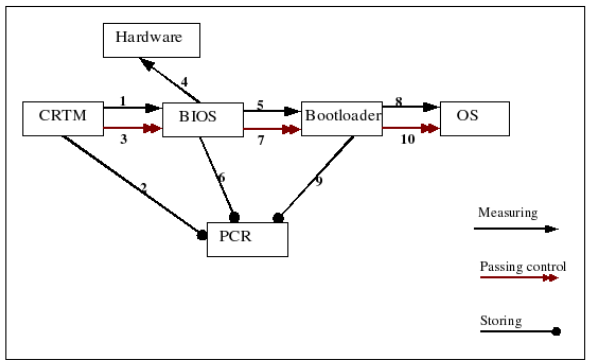
\includegraphics[scale=0.5]{img/trustedboot.png}
\end{wrapfigure}
\paragraph{Trusted Boot}\\
Questa si appoggia ad un co-processore crittografico (\emph{\textbf{TPM},Trusted Platform Module}) collocato sulla mainboard, con funzionalita' crittografiche e in grado quindi di verificare autenticita' e integrita', grazie anche a dati segreti ed immutabili contenuti internamente. In questo modo si evita di dipendere gia' dalla fase iniziale di software particolarmente complesso o di capacita' computazionali elevate e si demanda ad uno degli step configurabili intermedi la verifica tutti i precedenti passi siano stati svolti correttamente. Bisogna quindi avere a disposizione un BIOS o un Boot Loader che siano prima o poi in grado diverificare questi dati. Il sistema e' quindi pensato in maniera tale che materialmente il processo di boot possa procedere e non essere interrotto fintanto che non c'e' un componente sufficientemente sofisticato e con abbastanza capacita' algoritmica da poter controllare se i passi precedenti sono stati fatti correttamente. L'unica garanzia e' che anche se in precedenza sono stati eseguiti dei passi in maniera anomala , questi devono aver lasciato una traccia inalterabile di quel che e' successo. Quindi in qualche modo corro il rischio di aver fatto qualche passo attraverso software non affidabile , ma quest'ultimo di sicuro ha lasciato una traccia nel PCR indelebile in modo tale che quando arrivo ad un punto in cui e' possibile verificare gli step precedenti (\emph{applicazione, sistema operativo, boot loader}) verra' trovata una traccia di violazione di certe policy e agire di conseguenza. Questo si basa un po' sul fatto che a loro volta i componenti a valle non siano stati pesantemente alterati, rende comunque estremamente complesso (praticamente impossibile) arrivare abbastanza avanti nella catena da aver violato un'insieme tale di procedure di verifica in maniera che ignorino cio' che e' scritto nel PCR.


\begin{wrapfigure}{R}{6cm}
	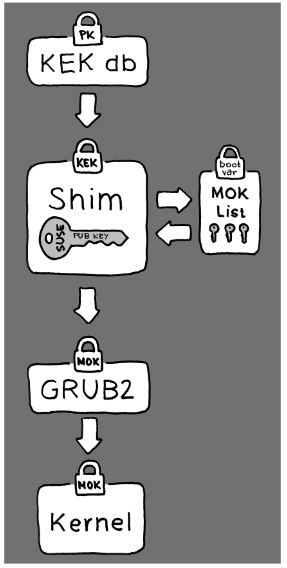
\includegraphics[scale=0.8]{img/secureboot.png}
\end{wrapfigure}
\paragraph{Secure Boot}\\
Questa tecnica si appoggia a UEFI, un sistema software piu' ampio e complesso pensato per sostituire interamente il BIOS tradizionale, che utilizza il minimo indispensabile, ovvero delle chiavi crittografiche utilizzate come elemento di verifica dell'integrita' e dell'autenticita' depositate nel firmware. Ovvero una parte fisica della memoria del sistema resa accessibili soltanto attraverso una procedura accuratamente controllata. UEFI nasce per sostituire completamente l'interfaccia fra sistema operativo e firmware, e' una specia di ``mini" sistema operativo che permtte di gestire i dischi in maniera enormemente piu' flessibile, e contiene un suo filesystem dedicato in cui conservare i bootloader. Questo fa delle verifiche a priori, ovvero impedisce materialmente ogni singolo step di boot se quello corrente non ha superato un controllo di autenticita' e integrita'. Si basa sul fatto che sul sistema sia installata una \textbf{Platform Key}, ovvero una chiave crittografica che permette di verifica se esiste sul sitema un piccolo componente, una sorta di bootloader di livello precedente a quello sopra descritto, verificato dall'hardware del BIOS utilizzando la platfom key. Questo standard e' stato sviluppato in collaborazione con Microsoft, che inizialmente era l'unica azienda a possedere le effettive chiavi,e quindi solo Microsoft poteva attestare l'autenticita' e quindi l'affidabilita' dei bootloader e dei sistemi operativi in maniera che venissero riconosciuti da \textbf{shim}. Questo avrebbe reso impossibile installare qualsiasi tipo di sistema operativo, che non fosse deciso da Microsoft, su qualsiasi sitema che adottava UEFI. 
Chiaramente cio' scateno' una quantita' di poliche non indifferenti a tal punto che Microsoft rispose immediatamente che non intendeva utilizzare questo meccanismo per limitare la liberta' degli utenti, e creo' un set di chiavi regalando alcune di queste ad altri produttori tra cui una alla Linux Foundation , un'ente no-profit che si occupa dell'ambiente Linux, con cui poter firmare i boot loader e le distribuzioni , cosi' che sia possibile utilizzare in armonia con EUFI. Ovviamente tutti i componenti, come abbiamo detto devono essere firmati, se intendo quindi modificare una parte del kernel, o di un qualsiasi altro componente dovro' poi crearne un'attestato (firma) sotto la mia responsabilita' valido solo per il mio sistema, che ne rappresenti l'autorizzazione per shim. 
\\
A tal scopo, esiste una gerarchia di chiavi, per cui io posso generarmi una chiave personale nota come \textbf{MOC, \emph{Machine Owner Key}} e con questa apporre un sigillo di autenticita' al software che intendo installare. A questo punto devo rendere riconoscibile la chiave, se intendo utilizzarla per validare l'autenticita' di un determinato componente, comunicandola a shim, e cio' e' possibile farlo in fase di pre-configurazione; sara' poi necessario un reboot ed un accesso fisico al terminale per autorizzare l'\emph{endowment}, ovvero il deposito effettivo della mia MOC all'interno della lista di MOC autorizzate. Si noti che si, questo database di chiavi puo' essere alterato, ma non a runtime e quindi da un eventuale software malevolo che va ad iniettare codice alterando il sistema di verifica perche' cio' necessita come detto un accesso fisico alla macchina.


\subsection{Hardening di secondo livello}
Visto le modalita' per un corretto avvio del sistema, comprese quelle piu attuali per garantire crittograficamente l'autenticita' e l'integrita' del boot loader e del sistema operativo , passiamo ad un secondo livello di ``\textbf{\emph{hardening}}" , ovvero il processo di messa in sicurezza e irrobustimento del sistema. Una volta appurata l'integrita' del sistema operativo, e' necessario configurarlo correttamente per far si' che l'\textbf{accesso alle risorse} segua il principio di \emph{\underline{minimo privilegio}} e il principio di \emph{\underline{negazione a priori}} di qualsiasi azione non esplicitamente autorizzata.

\subsubsection{Accesso alle risorse}
L'accesso alle risorse viene mediato dal sistema operativo; tutti i sistemi di accesso alle ricorse seguono una catena composta da 4 fasi:
\begin{itemize}
	\item \textbf{Identificazione}
	\item \textbf{Autenticazione}
	\item \textbf{Autorizzazione}
	\item \textbf{Auditing}
\end{itemize}

Dove l'\textbf{identificazione} permette di determinare quale e' il soggetto che richiede l'accesso. Normalmente questa fase viene incorporata con la fase successiva, ovvero quella di \textbf{autenticazione}, anche se in realta' le due fasi sono logicamente distinte: alcuni sistemi senza particolari esigenze di sicurezza posso funzionare benissimo basandosi su una semplice identificazione per consentire l'accesso a determinate risorse. Formalmente, l'\emph{identificazione} consente di capire qual sia il soggetto richiedende l'accesso, mentre l'\emph{autenticazione} mi permette di verificare se l'attestazione fatta dal soggetto propria identita' e' veriteria o meno. Una volta confermata l'identita' del soggetto, entra in gioco la fase di \textbf{Autorizzazione}: vado a determinare se questo puo' o no puo' eseguire determinate azioni sulle varie risorse messe a disposizione dal sistema (\emph{file, device, dispositivi fisici, interfacce di rete, etc}). 
Infine, la fase di \textbf{Auditing} che, dal punto di vista preditivo, non ha grande valenza. Se infatti voglio implementare una \emph{policy preditiva}, quindi che consenta l'utilizzo dell risorse solo a determinate categorie di utenti, devo agire attraverso i primi 3 step. Questo e' pero' il processo attraverso cui vengono \emph{tracciate} tutte le attivita' rilevanti o eventuali tentativi di svolgere determinate azioni da parte degli utenti (\emph{tentativi di autenticazione, esecuzione di operazioni di sistema, etc}) sulle risorse del sistema. Risulta particolarmente utile sia per controllare se vengono svolte attivita' illecite o sospette e quindi monitoraggio, sia per fare forensic post-illecito, ovvero consente di avere una traccia da analizzare attraverso la quale determinare quale delle decisioni progettuali o delle implementazioni di queste presentasse un'eventuale falla logica, consentendo quindi un'operazione non corretta.

\subsubsection{Autenticazione}
L'identificazione consiste semplicemente nel presentare qualche credenziale che puo' essere uno username o una caratteristica biometrica. Per quanto riguarda invece l'autenticazione, il soggetto richiedente, deve poter presentare un \textbf{dato non falsificabile} che viene con certezza associato alla sua identita' dal verificatore, che normalmente e' il sistema operativo. 
Il dato certo che ricerchiamo puo' assumere diverse forme:

\begin{itemize}
	\item ``\emph{Qualcosa che si e'}" \\
		conferma dell'identita' per confronto di una caratteristica intrinseca della persona, quindi fisiologica o comportamentale con un dato ``biometrico" di riferimento. Spesso nei sistemi biometrici (es. \emph{smartphone, sistema di unlock-door aziendale}), la fase di identificazione e autenticazione vengono collassate all'interno di un'unico step. Si pensi all'impronte digitale, questo puo' risultare in un eventuale problema di sicurezza in particolare in sistemi estesi, in quanto non solo deve capire se l'impronta presentata e' un'impronta corretta, ma deve farlo a fronte di un numero variabile e arbitrariamente alto di impronte pre-registrate con cui confrontarla. Questo porta, per un eventuale attaccante, ad un aumento della probabilita' che presentando la propria impronta, questa venga confusa con almeno una fra quelle autorizzate, di fatto creando una situazione molto piu' favorevole paragonata ad un contesto in cui indentificazione e autorizzazione sono invece separate, dato che se dichiaro in primis una determinata identita', e poi cerco di autenticarla, avro' un solo possibile campione, con cui confrontare quello che tento di inserire diminuendo drasticamente la possibilita' di falsi positivi. Un'altra problematica legata ai dati biometrici e' che questi sono, per loro natura, soggetti ad un alto livello di ``\emph{rumore}" per cui un margine di errore deve essere per forza tenuto in considerazione , altrimenti all'opposto rischio di generare una grande quantita' di falsi negativi, ovvero di rifiuti di autenticazione a fronte di dati biometrici corretti.

	\item ``\emph{Qualcosa che si ha}"\\
		e' il processo di conferma dell'identita' attraverso il possesso di un oggetto fisico , che deve quindi esssere custodito attentamente, riconoscibile da parte della macchina che effettua il controllo (\emph{scheda a banda magnetica, smart card, token RFID, smartphone, etc\dots})

	\item ``\emph{Qualcosa che si sa}"\\
		conferma dell'identita' dimostrando la conoscenza di un dato segreto concordato in precedenza (\emph{password, Personal Identification Number - PIN, una chiave, etc\dots}), dove il problema e' che per esser veramente affidabile dovrebbe essere effettivamente un dato ricordato a memoria e non presente su qualsiai dispositivo fisico.
\end{itemize}

\subsubsection{Gestione degli utenti}
Nessun sistema e' completo senza dei meccanismi di sicurezza. Dev'essere presente un meccanismo per proteggere i file da letture o modifiche non autorizzate. Il sistema Linux si accosta  alla metodologia di UNIX attribuendo permessi ai file, permettendo ad utenti singoli e gruppi l'accesso ai file sulla base di un insieme di permessi di sicurezza per ogni file e directory. Gli account utente sono un ingranaggio fondamentale di questo meccanismo. Ogni individuo che accede ad un sistema linux deve essere in possesso di un account utente univoco. I permessi che quest'ultimo avra' sui vari oggetti nel sistema dipendera' dall'identita' che assume internamente al sistema.

I permessi utente vengono tracciati attraverso uno \textbf{user ID} (\emph{UID}), assegnato ad un account al momento della creazione. Questo e' un vaore numerico, univoco per ogni utente. Ad ogni modo per accedere al sistema, non viene utilizzato lo user ID, bensi' un \textbf{login name}. Questo e' una stringa alfanumerica di 8 o meno caratteri che l'utente puo' utilizzare per fare log in nel sistema (generalmente insieme ad una password associata)

Linux si appoggia a file ed utility speciali per gestire e monitorare gli account utenti all'interno del sistema.Vediamo alcuni degli elementi principali che partecipano in questo meccanismo:

\paragraph{\texttt{/etc/passwd}} Il Sistema si appoggia ad un file speciale per controllare le corrispondenze tra \emph{login name} e \emph{UID}: il file \texttt{/etc/passwd}. Questo contiene diversi pezzi di informazione riguardanti tutti gli utenti presenti all'interno del sistema.

\begin{lstlisting}[language=bash,basicstyle=\ttfamily,frame=single,caption={Struttura di un file /etc/passwd},captionpos=b]
$ cat \etc\passwd
root:x:0:0::/root:/bin/bash
bin:x:1:1::/:/sbin/nologin
daemon:x:2:2::/:/sbin/nologin
mail:x:8:12::/var/spool/mail:/sbin/nologin
ftp:x:14:11::/srv/ftp:/sbin/nologin
http:x:33:33::/srv/http:/sbin/nologin
nobody:x:65534:65534:Nobody:/:/sbin/nologin
dbus:x:81:81:System Message Bus:/:/sbin/nologin
elliot:x:1001:1001:Elliot:/home/elliot:/bin/bash
\end{lstlisting}

Gli utenti e i gruppi possono essere creati rispettivamente utilizzando i comandi: \texttt{useradd} e \texttt{addgroup}. Entrambi i comandi supportano varie opzioni consultabili 

\subsubsection{Password}

